\documentclass[graphics]{beamer}
\usepackage{xcolor}
\usepackage{graphicx}
\usepackage{verbatim}
\usepackage{wrapfig}
\useoutertheme{shadow}
%\usecolortheme{orchid}
\usecolortheme{seahorse}


% math commands
\newcommand{\be}{\begin{eqnarray}}
\newcommand{\ee}{\end{eqnarray}}
\newcommand{\beq}{\begin{equation}}
\newcommand{\eeq}{\end{equation}}
\def\simless{\mathbin{\lower 3pt\hbox
      {$\rlap{\raise 5pt\hbox{$\char'074$}}\mathchar"7218$}}}
\def\simgreat{\mathbin{\lower 3pt\hbox
      {$\rlap{\raise 5pt\hbox{$\char'076$}}\mathchar"7218$}}} %> or of order

% variables

\def\toonscale{0.45}
\def\mboxy#1{\mbox{\small #1}}

\defbeamertemplate*{title page}{customized}[1][]
{
  \usebeamerfont{title}\inserttitle\par
  \usebeamerfont{subtitle}\usebeamercolor[fg]{subtitle}\insertsubtitle\par
  \bigskip
  \usebeamerfont{author}\insertauthor\par
  \usebeamerfont{institute}\insertinstitute\par
  \usebeamerfont{date}\insertdate\par
  \usebeamercolor[fg]{titlegraphic}\inserttitlegraphic
}
\begin{comment}
\AtBeginSection[]{
  \frame{
    \frametitle{Outline}
    \tableofcontents[currentsection]
  }
}
\end{comment}


\title{Fast Radio Bursts}
%\subtitle{}
\author[U. Pen]{{
\textcolor{green}{\small K. Masui, H-S. Lin, J. Sievers}, 
\textcolor{cyan}{\small Y. Li, Y. Jadav, L. Connor} 
\textcolor{darkgray}{\small U. Pen, X. Chen, J. Peterson and many more}
}
\\[8mm] 
}
\date{December 24, 2015}


\begin{document}

\frame{
\vspace{-0.5in}
\begin{center}  
%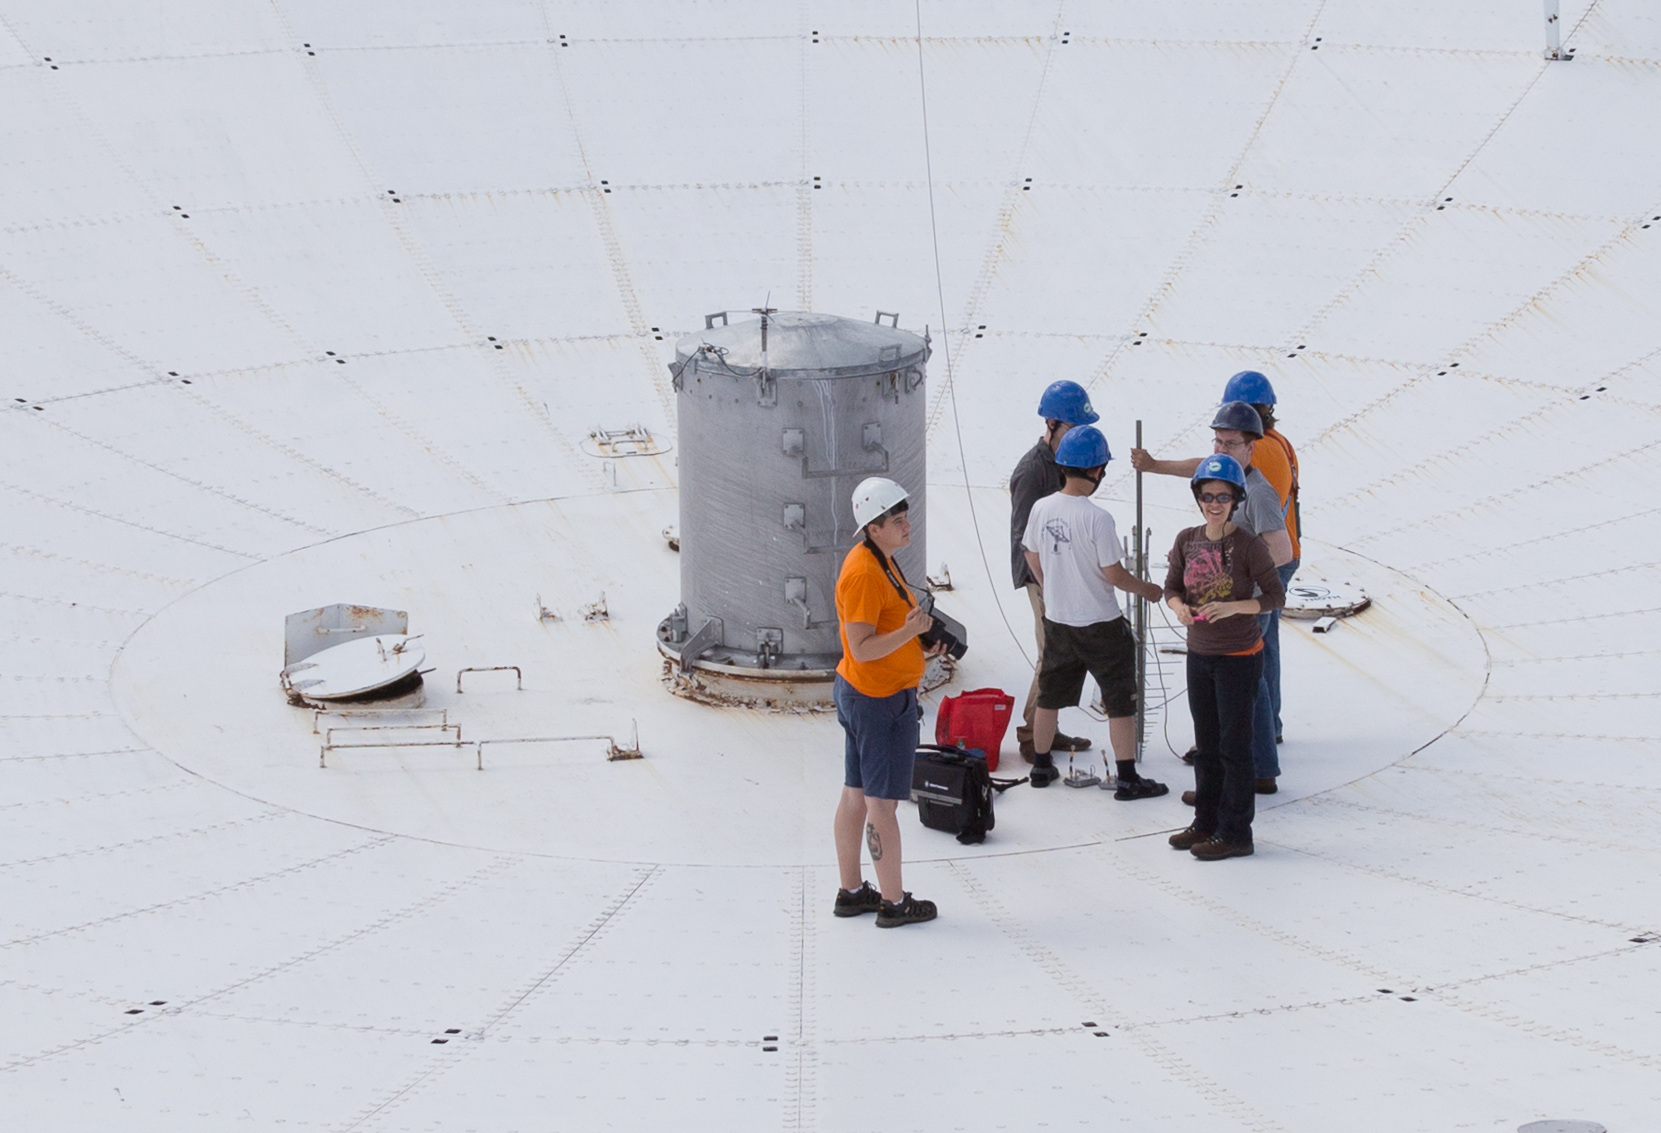
\includegraphics[width=4.4in]{Figures/IMG-0438-by-Andre-cropped.jpg}
\end{center}
\begin{picture}(320,250)
\put(-50,60){
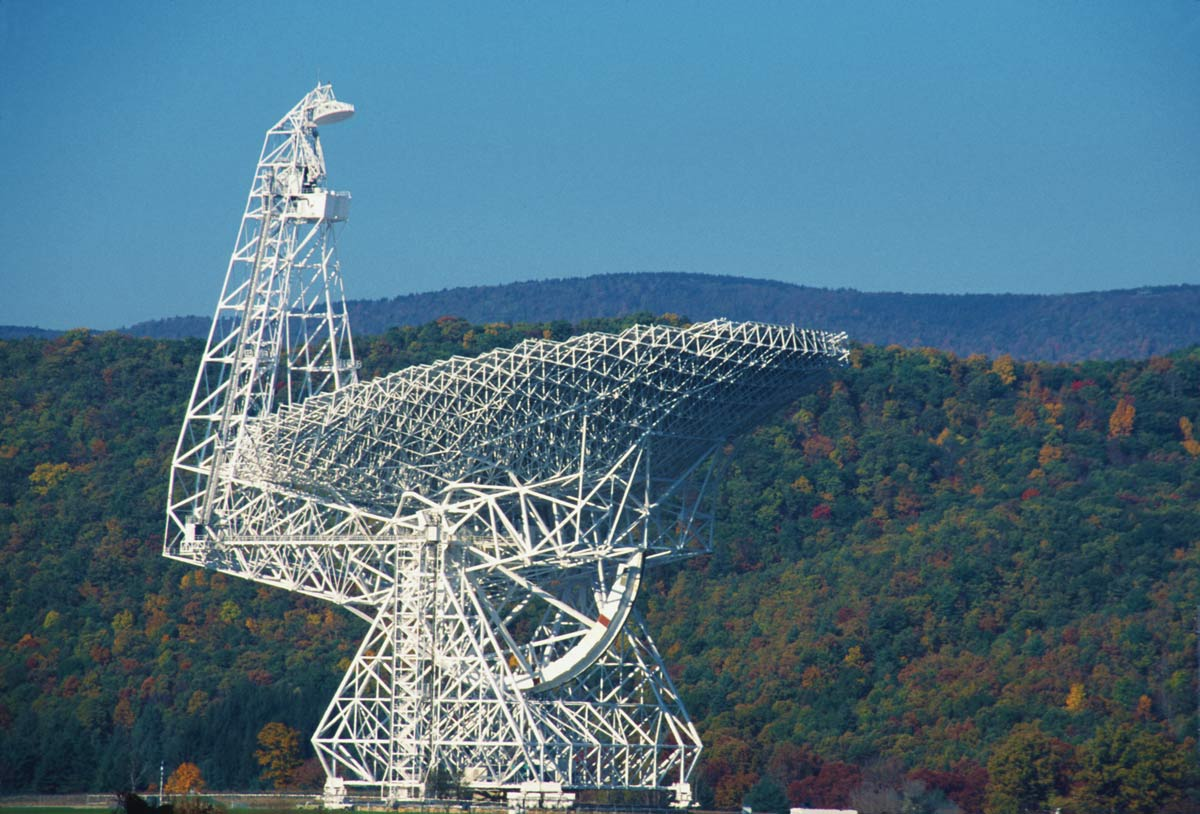
\includegraphics[width=5.5in]{Figures/GBT_nrao.jpg}}
\end{picture}
\vspace{-4in}
\\
image credit: NRAO/AUI/NSF
\\
\vspace{1in}
\titlepage
}

%\section*{Introduction}
\section{Introduction}

\begin{comment}
  \subsection{Outline}

  \frame{
    \frametitle{Outline}
    \tableofcontents
  }
\end{comment}

  \frame{
    \frametitle{Overview}
    \begin{itemize}
      \item FRB
      \item Candidates
      \item Plasma Lensing
      \item Controversies
      \item next steps
    \end{itemize}
  }
\section{FRBs}

\frame{
    \frametitle{FRB}
     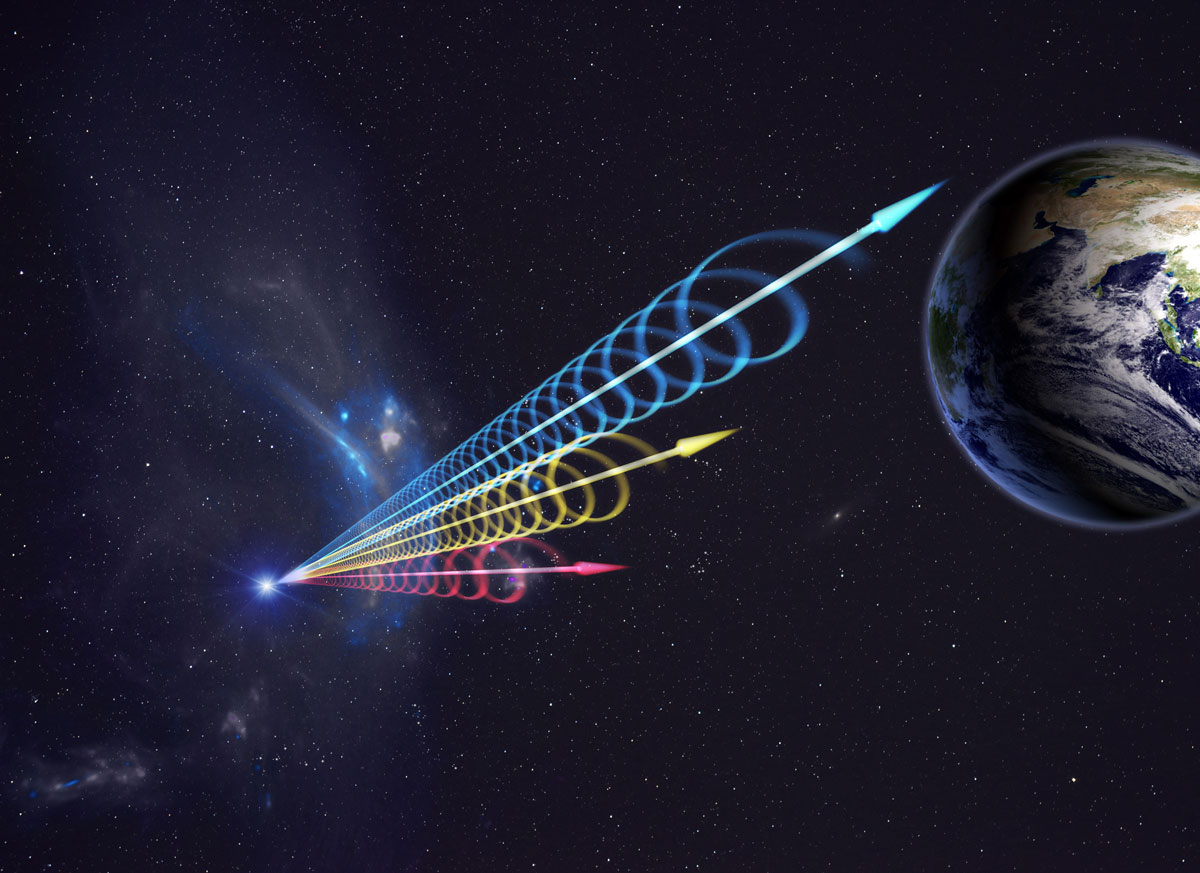
\includegraphics[width=\textwidth]{Figures/FRB_nrao.jpg}
}


  \frame{
    \frametitle{Basic Properties}
    \begin{itemize}
      \item about 20 FRBs detected
      \item ms duration
      \item some are scattered
      \item some are polarized
      \item high dispersion measure: DM $\sim$ 1000 pc/cm$^3$
      \item likely extragalactic
      \item possibly cosmological $z\sim 1$
      \item R-J brightness: $10^{36}$K is $\sim 10^4 T_p$ 
    \end{itemize}
  }


  \frame{
    \frametitle{Candidates}
    \begin{itemize}
      \item cataclysmic: exploding hawking black holes, merging
        neutron stars
      \item repeating: magnetars, planet-neutron star, supergiant flare
      \item local: flare stars, microwave ovens
    \end{itemize}
  }


  \frame{
    \frametitle{FRB110523}
    \begin{itemize}
    \item Masui et al, Dec 2, 2015, Nature 15769
    \item  recorded on May 23, 2011
     \item GBT-IM survey, for 21cm intensity mapping (Chang et al 2010,
       Nature, 466, 463)
     \item beat double odds with data: intensity mapping, FRB       
    \end{itemize}
  }
\frame{
    \frametitle{Waterfall}
     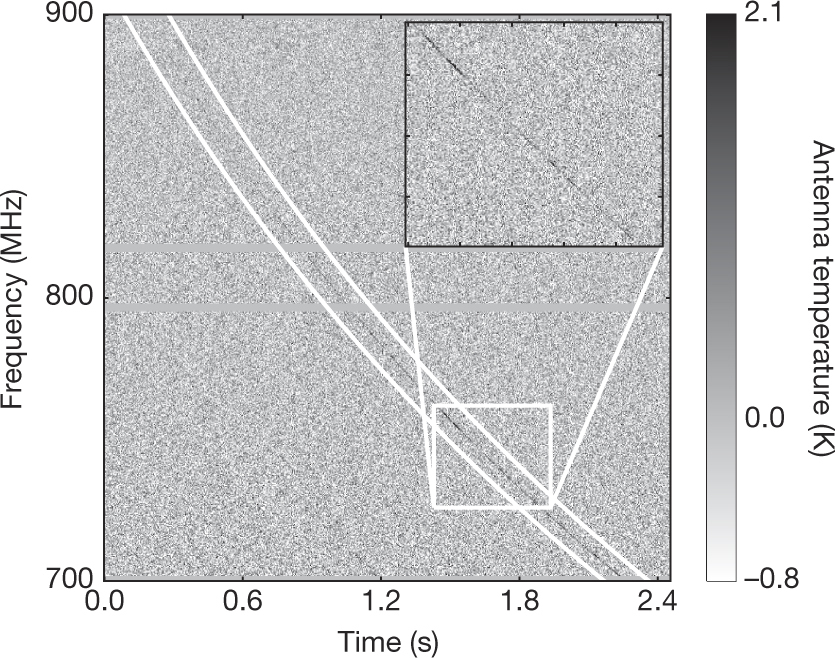
\includegraphics[width=0.8\textwidth]{Figures/nature15769-f1.jpg}
}
\frame{
    \frametitle{Polarization}
     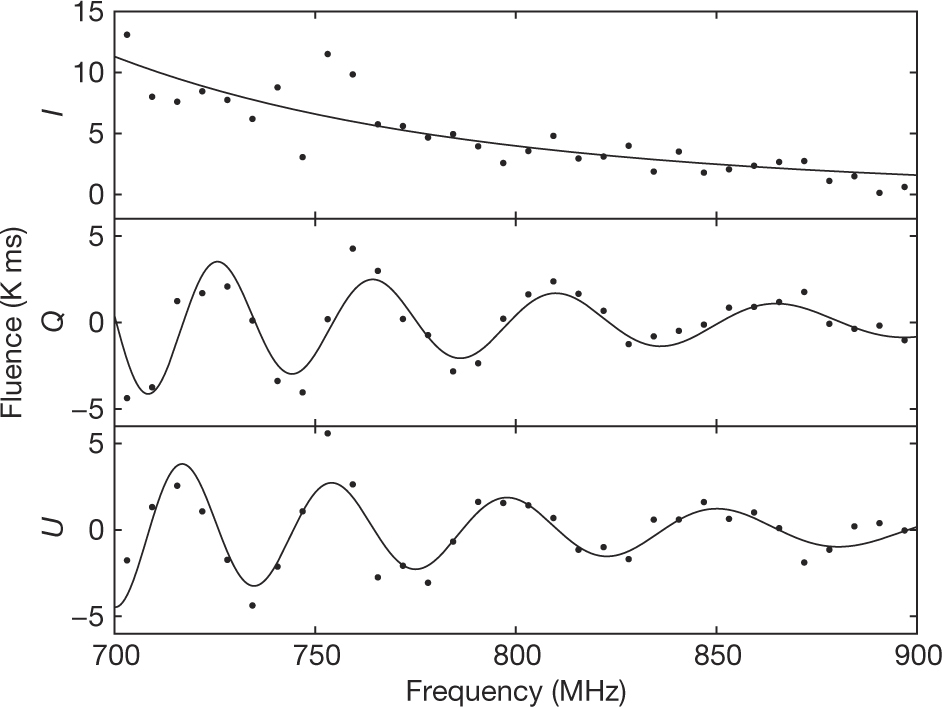
\includegraphics[width=0.8\textwidth]{Figures/nature15769-f2.jpg}
}
\frame{
    \frametitle{Angle swing}
     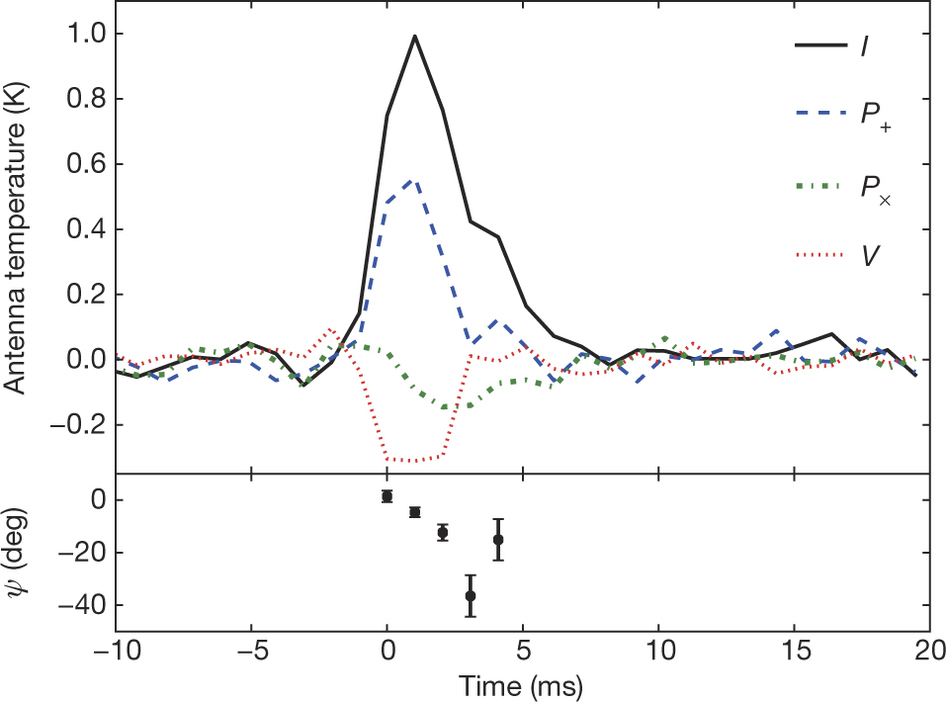
\includegraphics[width=0.8\textwidth]{Figures/nature15769-f3.jpg}
}
\frame{
    \frametitle{Scattering}
     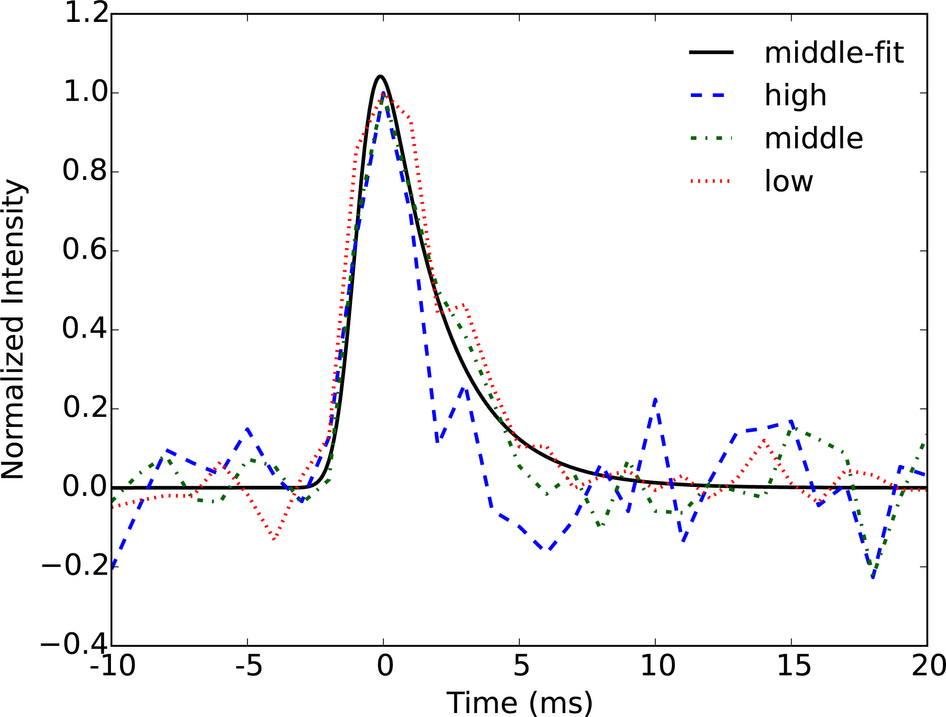
\includegraphics[width=0.8\textwidth]{Figures/nature15769-sf2.jpg}
}
\frame{
    \frametitle{inferred properties}
     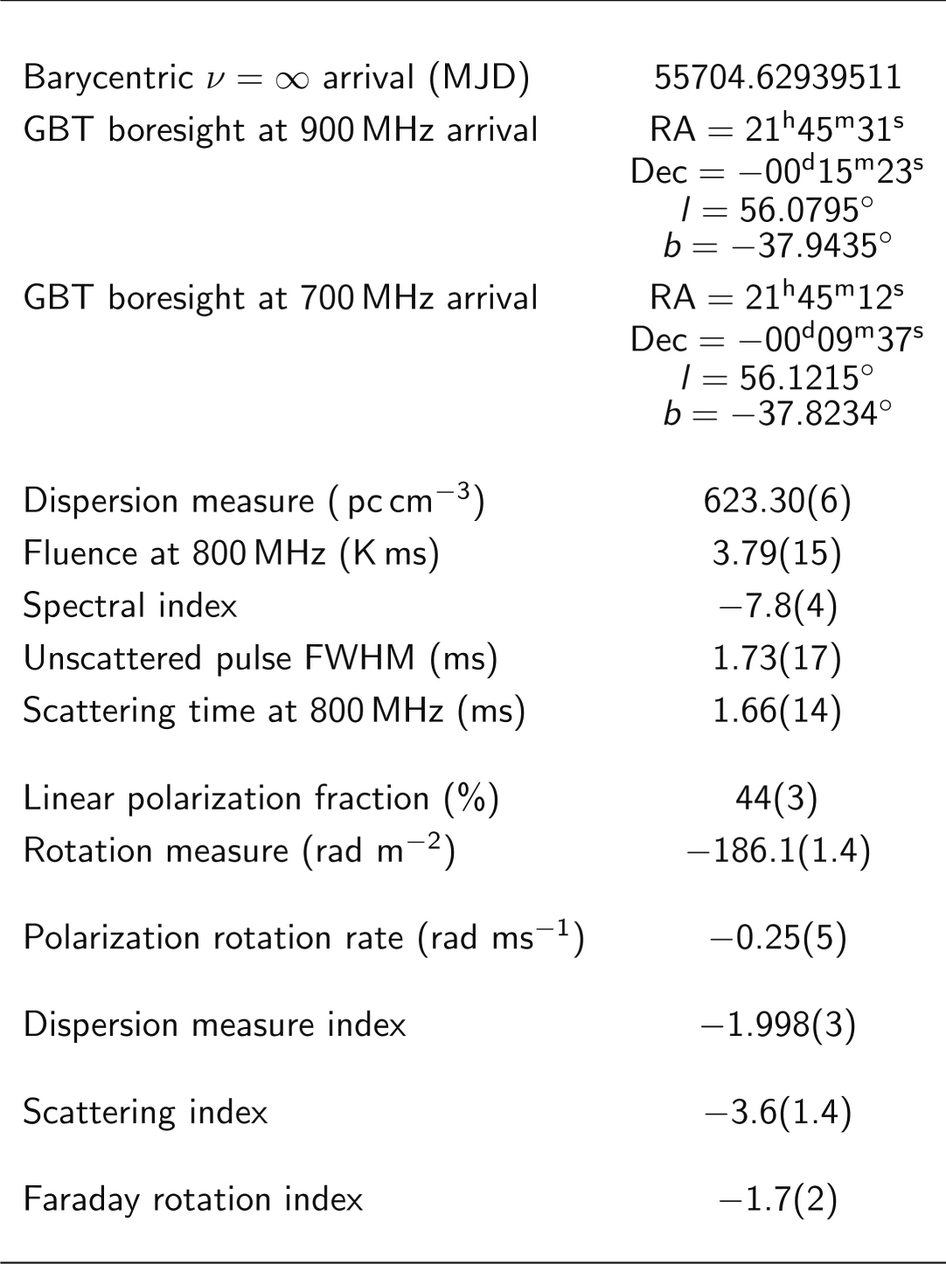
\includegraphics[width=0.8\textwidth]{Figures/nature15769-st1.jpg}
}

\section{Summary}
  \frame{
    \frametitle{Looking forward}
    \begin{itemize}
      \item more unpublished bursts with new measurements
      \item thousands of bursts with CHIME, HIRAX, UTMOST
      \item localization with VLBI
      \item 
      \item 
    \end{itemize}
  }


  \frame{
    \frametitle{Speculation}
    \begin{itemize}
    \item grazing incidence reconnection sheets
    \item ULP + Levin 2014
    \item ULP + King 2012
    \item Liu + ULP 2015
    \item 1-D structure
    \item localized scattering
%    \item predicts RM gradient
    \end{itemize}
\begin{picture}(320,235)
\put(110,170){
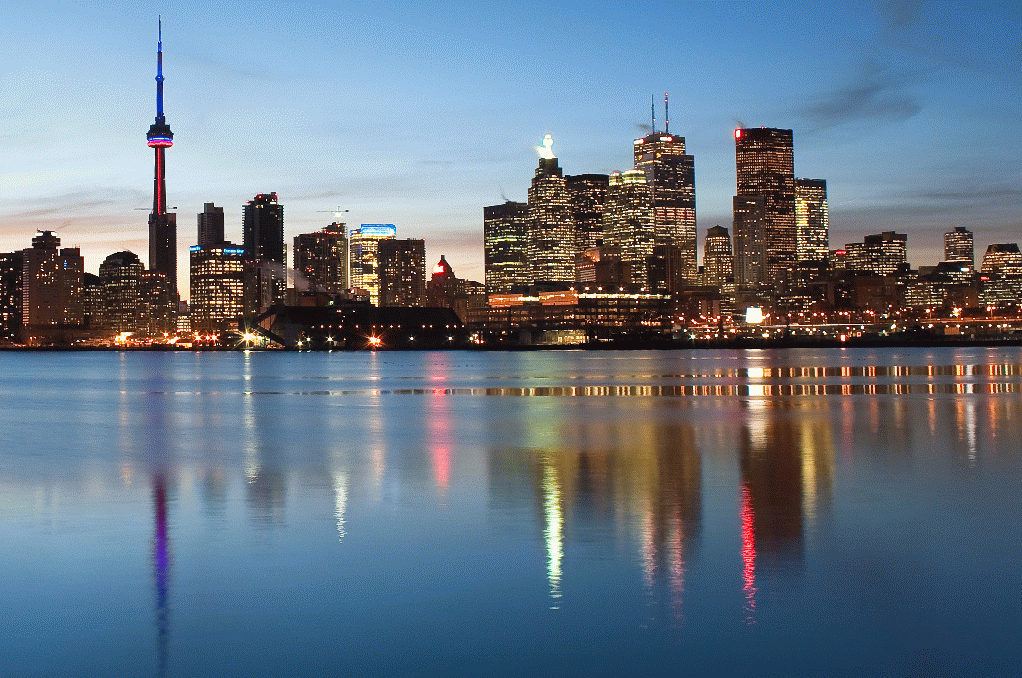
\includegraphics[width=3.0in]{Figures/toronto-skyline.png}}
\put(-60,-207){
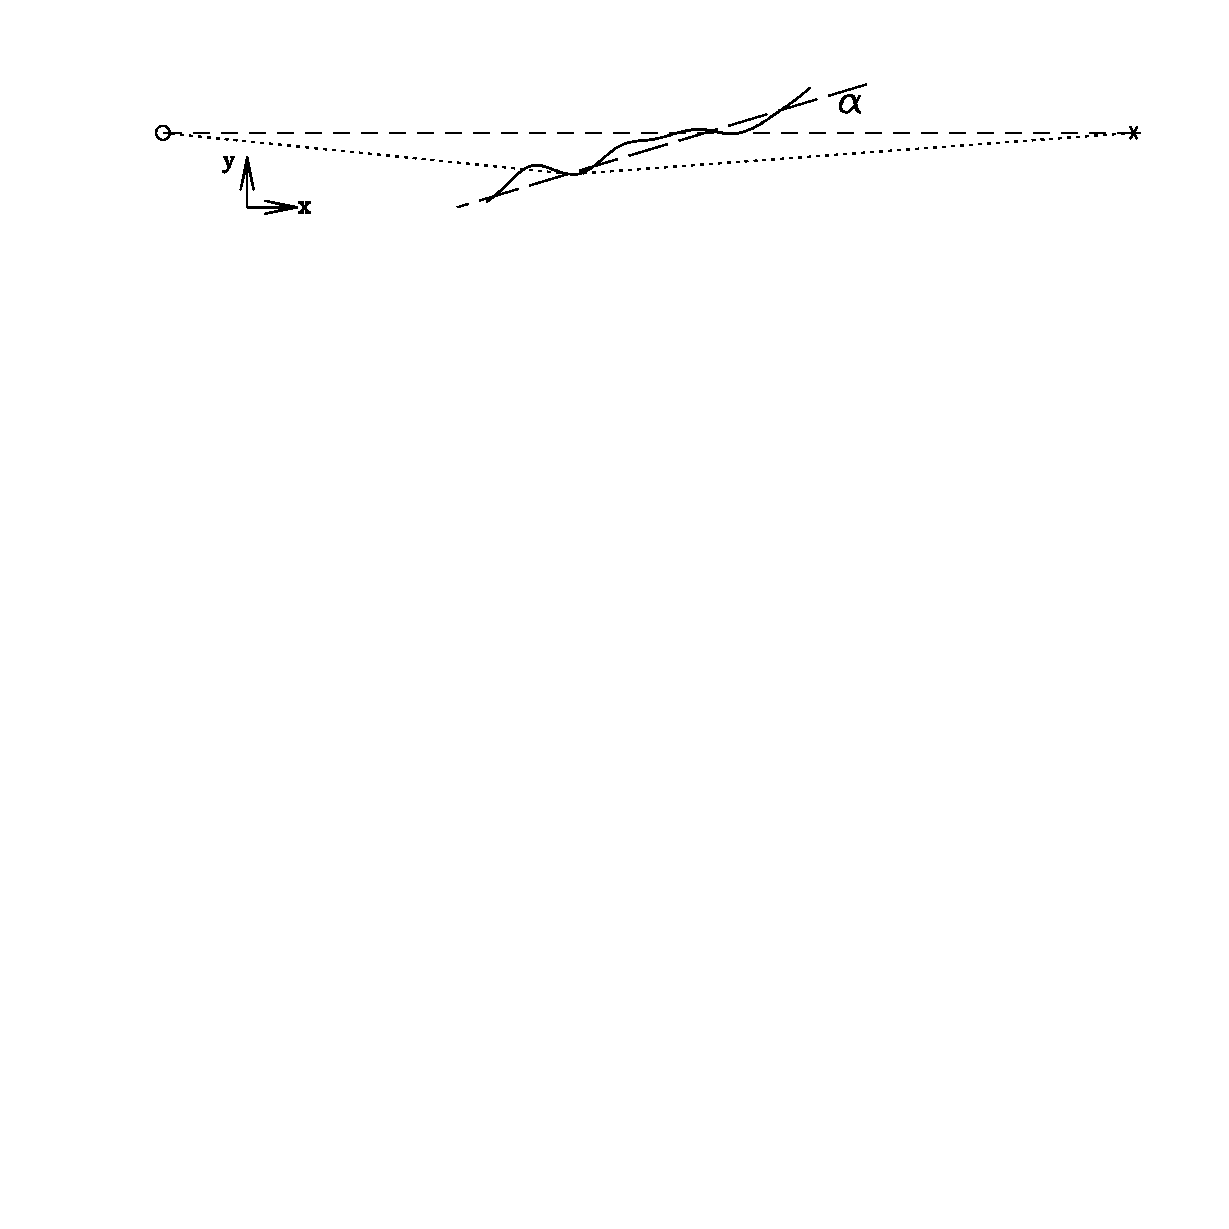
\includegraphics[width=5.5in]{Figures/sheetgeom.eps}}
\end{picture}
  }
  \frame{
    \frametitle{Folds}
\begin{center}
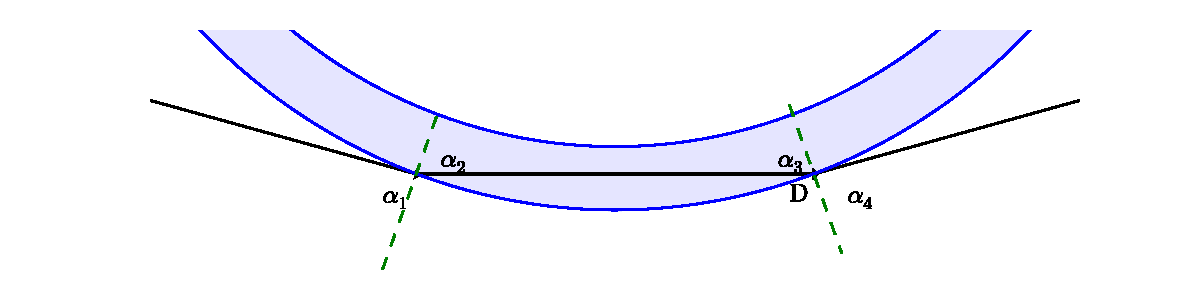
\includegraphics[width=3.9in]{Figures/refraction.pdf}
\end{center}

Refraction of light rays near point D.  The black lines
  are the light paths.  The shaded region indicates the lensing sheet
  caustic.  The angles obey Snell's Law
  $\frac{\sin(\alpha_1)}{\sin(\alpha_2)}=\frac{\sin(\alpha_4)}{\sin(\alpha_3)}=\frac{n_{\rm sheet}}{n_{\rm
    ISM}.$ }
}



  \frame{
    \frametitle{Conclusion}
    \begin{itemize}
      \item FRBs: 
      \item PTA pulsar distance: new precision window for gravitational wave astronomy
      \item Pulsar magnetosphere mapping: matter in extreme conditions
      \item ISM structure: mapping cosmic plasma and magnetic fields
    \end{itemize}
  }

\end{document}
